\section{}
A uniform bar of rectangular cross section $2h \times b$ and specific weight $\gamma$ hangs in the vertical plane
as shown in Fig. \ref{fig:Q5}. Its weight results in displacements shown below. Demonstrate whether
this solution satisfies the 15 equations of elasticity and the boundary conditions.

\begin{figure}[h]
    \centering
    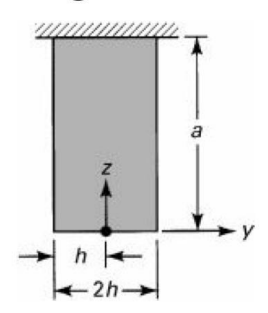
\includegraphics[width=0.5\linewidth]{Questions/Figures/Q5ProblemDiagram.png}
    \caption{Uniform rectangular bar.}
    \label{fig:Q5}
\end{figure}

\begin{align*}
    u &= \frac{-\nu\gamma}{E} xz \\
    v &= \frac{-\nu\gamma}{E} yz \\
    w &= \frac{\gamma}{2E} \left[\frac{z^2 - a^2) + \nu(x^2 + y^2)}{2}\right]
\end{align*}

\textbf{Solution}
First calculate the strains from the displacements (6 equations):
\[
\begin{aligned}
    \epsilon_x &= \frac{\partial u}{\partial x} = \frac{-\nu\gamma}{E} z \\
    \epsilon_y &= \frac{\partial v}{\partial y} = \frac{-\nu\gamma}{E} z \\
    \epsilon_z &= \frac{\partial w}{\partial z} = \frac{\gamma}{E} z \\
    \gamma_{xy} &= \frac{\partial u}{\partial y} + \frac{\partial v}{\partial x} = 0 \\
    \gamma_{yz} &= \frac{\partial v}{\partial z} + \frac{\partial w}{\partial y} = 0 \\
    \gamma_{xz} &= \frac{\partial u}{\partial z} + \frac{\partial w}{\partial x} = 0 \\\
\end{aligned}
\]

Next, check compatibility (6 equations):
\[
\begin{aligned}
    \frac{\partial^2 \gamma_{xy}}{\partial x \partial y} &= \frac{\partial^2 \epsilon_x}{\partial y^2} + \frac{\partial^2 \epsilon_y}{\partial x^2} \\
    \frac{\partial^2}{\partial x \partial y} 0 &= \frac{\partial^2}{\partial y^2} \frac{-\nu\gamma}{E} z + \frac{\partial^2}{\partial x^2} \frac{-\nu\gamma}{E} z \\
    0 &= 0 + 0 \\
\end{aligned}
\]

\[
\begin{aligned}
    \frac{\partial^2 \gamma_{xz}}{\partial x \partial z} &= \frac{\partial^2 \epsilon_x}{\partial z^2} + \frac{\partial^2 \epsilon_z}{\partial x^2} \\
    \frac{\partial^2}{\partial x \partial z} 0 &= \frac{\partial^2}{\partial z^2} \frac{-\nu\gamma}{E} z + \frac{\partial^2}{\partial x^2} \frac{\gamma}{E} z \\
    0 &= 0 + 0 \\
\end{aligned}
\]  

\[
\begin{aligned}
    \frac{\partial^2 \gamma_{yz}}{\partial y \partial z} &= \frac{\partial^2 \epsilon_y}{\partial z^2} + \frac{\partial^2 \epsilon_z}{\partial y^2} \\
    \frac{\partial^2}{\partial y \partial z} 0 &= \frac{\partial^2}{\partial z^2} \frac{-\nu\gamma}{E} z + \frac{\partial^2}{\partial y^2} \frac{\gamma}{E} z \\
    0 &= 0 + 0 \\
\end{aligned}
\]

\[
\begin{aligned}
    \frac{\partial}{\partial x} \left(\frac{\partial \epsilon_xy}{\partial z}  + \frac{\partial \epsilon_xz}{\partial y} - 
    \frac{\partial \epsilon_yz}{\partial x}\right) &= \frac{\partial^2 \epsilon_x}{\partial y \partial z}\\
    \frac{\partial}{\partial x} \left(\frac{\partial}{\partial z} 0  + \frac{\partial}{\partial y} 0 - 
    \frac{\partial}{\partial x} 0\right) &= \frac{\partial^2}{\partial y \partial z} \frac{-\nu\gamma}{E} z \\
    0 &= 0 \\
\end{aligned}
\]

\[
\begin{aligned}
    \frac{\partial}{\partial y} \left(\frac{\partial \epsilon_xy}{\partial z}  + \frac{\partial \epsilon_xz}{\partial y} - 
    \frac{\partial \epsilon_yz}{\partial x}\right) &= \frac{\partial^2 \epsilon_y}{\partial x \partial z}\\
    \frac{\partial}{\partial y} \left(\frac{\partial}{\partial z} 0  + \frac{\partial}{\partial y} 0 - 
    \frac{\partial}{\partial x} 0\right) &= \frac{\partial^2}{\partial x \partial z} \frac{-\nu\gamma}{E} z \\
    0 &= 0 \\
\end{aligned}
\]

\[
\begin{aligned}
    \frac{\partial}{\partial z} \left(\frac{\partial \epsilon_xy}{\partial z}  + \frac{\partial \epsilon_xz}{\partial y} - 
    \frac{\partial \epsilon_yz}{\partial x}\right) &= \frac{\partial^2 \epsilon_z}{\partial x \partial y}\\
    \frac{\partial}{\partial z} \left(\frac{\partial}{\partial z} 0  + \frac{\partial}{\partial y} 0 - 
    \frac{\partial}{\partial x} 0\right) &= \frac{\partial^2}{\partial x \partial y} \frac{\gamma}{E} z \\
    0 &= 0 \\
\end{aligned}
\]

Finally, check equilibrium (3 equations):
\[
\begin{aligned}
    \frac{\partial \sigma_{x}}{\partial x} + \frac{\partial \tau_{xy}}{\partial y} + \frac{\partial \tau_{xz}}{\partial z} + F_x &= 0 \\
    \frac{\partial \tau_{yx}}{\partial x} + \frac{\partial \sigma_{y}}{\partial y} + \frac{\partial \tau_{yz}}{\partial z} + F_y &= 0 \\
    \frac{\partial \tau_{zx}}{\partial x} + \frac{\partial \tau_{zy}}{\partial y} + \frac{\partial \sigma_{z}}{\partial z} + F_z &= 0 \\
\end{aligned}
\]

Using Lame's equations,
\[
\begin{aligned}
    \lambda &=  \frac{E\nu}{(1 + \nu)(1 - 2\nu)} \\
    e &= \epsilon_x + \epsilon_y + \epsilon_z \\
    &= \frac{-\nu\gamma}{E} z + \frac{-\nu\gamma}{E} z + \frac{\gamma}{E} z \\
    &= \frac{z\gamma}{E} (1 - 2\nu) \\
\end{aligned}
\]

Also note since shear strains are zero, $\tau_{xy} = \tau_{xz} = \tau_{yz} = 0$ by the relation $\tau = G\gamma$. Also there 
are no body forces, $F_x = F_y = F_z = 0$.
The equilibrium equations reduce:
\[
\begin{aligned}
    \frac{\partial \sigma_{x}}{\partial x} &= \\
    0 &= \frac{\partial}{\partial x} (2G \epsilon_x + \lambda e) \\
    0 &= \frac{\partial}{\partial x} (2G \frac{-\nu\gamma}{E} z + \lambda \frac{z\gamma}{E} (1 - 2\nu)) \\
    0 &= 0 \\
\end{aligned}
\]

\[
\begin{aligned}
    \frac{\partial \sigma_{y}}{\partial y} &=  \\
    0 &= \frac{\partial}{\partial y} (2G \epsilon_y + \lambda e)  \\
    0 &= \frac{\partial}{\partial y} (2G \frac{-\nu\gamma}{E} z + \lambda \frac{z\gamma}{E} (1 - 2\nu)) \\
    0 &= 0 \\
\end{aligned}
\]

\[
\begin{aligned}
    \frac{\partial \sigma_{z}}{\partial z} &=  \\
    0 &= \frac{\partial}{\partial z} (2G \epsilon_z + \lambda e)  \\
    0 &= \frac{\partial}{\partial z} (2G \frac{\gamma}{E} z +  \frac{z\gamma}{E} (1 - 2\nu)) \\
    0 &= 0 \\
\end{aligned}
\]